\documentclass{article}

\usepackage[utf8]{inputenc}
\usepackage{amsthm}
\usepackage{amssymb}
\usepackage{mathtools}
\usepackage{graphicx}
\usepackage{mdframed}
\usepackage{float}
\usepackage[top=0.75in, bottom=0.75in, left=0.75in, right=0.75in]{geometry}
\usepackage{gauss}

\usepackage{array}
\allowdisplaybreaks

\makeatletter
\newcounter{elimination@steps}
\newcolumntype{R}[1]{>{\raggedleft\arraybackslash$}p{#1}<{$}}
\def\elimination@num@rights{}
\def\elimination@num@variables{}
\def\elimination@col@width{}
\newenvironment{elimination}[4][0]
{
    \setcounter{elimination@steps}{0}
    \def\elimination@num@rights{#1}
    \def\elimination@num@variables{#2}
    \def\elimination@col@width{#3}
    \renewcommand{\arraystretch}{#4}
    \start@align\@ne\st@rredtrue\m@ne
}
{
    \endalign
    \ignorespacesafterend
}
\newcommand{\step}[2]
{
    \ifnum\value{elimination@steps}>0\sim\quad\fi
    \left[
        \ifnum\elimination@num@rights>0
            \begin{array}
            {@{}*{\elimination@num@variables}{R{\elimination@col@width}}
            |@{}*{\elimination@num@rights}{R{\elimination@col@width}}}
        \else
            \begin{array}
            {@{}*{\elimination@num@variables}{R{\elimination@col@width}}}
        \fi
            #1
        \end{array}
    \right]
    & 
    \begin{array}{l}
        #2
    \end{array}
    \addtocounter{elimination@steps}{1}
}
\makeatother

\DeclarePairedDelimiter{\abs}{\lvert}{\rvert}
\DeclarePairedDelimiter{\norm}{\lvert \lvert}{\rvert \rvert}

\newtheoremstyle{break}% name
  {}%         Space above, empty = `usual value'
  {}%         Space below
  {\itshape}% Body font
  {}%         Indent amount (empty = no indent, \parindent = para indent)
  {\bfseries}% Thm head font
  {.}%        Punctuation after thm head
  {\newline}% Space after thm head: \newline = linebreak
  {}%         Thm head spec

\newtheorem{Def}{Definition}[section]

\theoremstyle{break}

\newtheorem{innerEx}{Exempel}[section]
\newtheorem{sats}{Sats}[section]
\newtheorem{Rem}{Anmärkning}[]

\newenvironment{Ex}
{\begin{mdframed} \begin{innerEx} \vspace{3pt}}
{\vspace{3pt} \end{innerEx} \end{mdframed}}  

\newenvironment{bevis}
{\begin{mdframed} \begin{proof} \vspace{3pt}}
{\vspace{3pt} \end{proof} \end{mdframed}}


\title{
	 Linjär Algebra\\
	 Föreläsning 18
    \author{Erik Sjöström}
}
\begin{document}
\maketitle

\section{Egenvärdensproblemet som linjär avbildning} % (fold)
\label{sec:egenv_rdensproblemet_som_linj_r_avbildning}
\begin{align*}
&f : \mathbb{R}^n \rightarrow \mathbb{R}^n
&&f(\vec{x}) = \mathbf{A} \cdot \vec{x}
\end{align*}
\noindent
Man ställer sig frågan: Vilka $\vec{x}$ avbildas på $\lambda \cdot \vec{x}$?
\[
	\mathbf{A} \cdot \vec{x} = \lambda \cdot \vec{x}
\]
\begin{Ex}
	Projektion (se lab 4) på ett plan $\pi$:
	\[
	a \cdot \vec{x} + b \cdot \vec{y} + c \cdot \vec{z} = 0 \mbox{ ,genom origo}
	\]
	är en linjär avbildning och kan skrivas som:
	\[
	\vec{x}_{\pi} = \mathbf{A} \cdot \vec{x}
	\]
	Egenvärden, egenvektorer till \textbf{A}?
	\begin{itemize}
		\item Alla vektorer $\vec{x}_{\pi}$ i planet kommer att vara offörändrade så de kommer att vara egenvektorer med egenvärde 1.
		\[
		1 \cdot \vec{x}_{\pi} = \mathbf{A} \cdot \vec{x}_{\pi}
		\]
		\item Alla vektorer vinkelräta mot planet (dvs: parallella med normalen $\vec{n}$).
		\[
		\mathbf{A} \cdot \vec{n} = 0 \cdot \vec{n} 
		\]
		dvs: $\vec{n}$ egenvektor med egenvärde 0.  
	\end{itemize}
\end{Ex}
\begin{Ex}
	Spegling genom plan som går genom origo är en linjär avbildning: $f(\vec{x}) = \mathbf{A} \cdot \vec{x}$
	\begin{itemize}
		\item Alla $\vec{x}_{\pi}$ i planet förblir oförändrade, dvs de är egenvektorer med egenvärde 1.
		\item Alla vektorer vinkelräta mot planet (parallell med $\vec{n}$)  har spegelbild den vektor som är lika lång och pekar i motsatt riktning, dvs $\vec{n}$ är egenvektor med egenvärde -1:
		\[
		\mathbf{A} \cdot \vec{n} = -1 \cdot \vec{n}
		\]
	\end{itemize}
\end{Ex}
% section egenv_rden_och_egenv_rdensproblem (end)

\section{Grafer} % (fold)
\label{sec:grafer}
\begin{Def}
	En graf $\mathbf{G} = (\mathbf{V}, \mathbf{R})$ består av noder \textbf{V}, och kanter \textbf{E}. Kanterna består av oordnade element $\{v_i, v_j\}$ ur \textbf{V}. Om grafen är riktad så består \textbf{E} av ordnade par $(v_i, v_j)$\\
	Graden $d(v_i)$ för en nod $v_i$ är antalet grannar till $v_i$
\end{Def}
\begin{Def}
	Låt $\mathbf{G} = (\mathbf{V}, \mathbf{E})$ vara en graf med \textit{n} noder. Elementen i grannmatrisen $\mathbf{A}_{G}$ ges av:
	\begin{align*}
	&a_{ij} = 
	\begin{cases}
		1 &\mbox{ om } \{v_i, v_j\} \\
		0 &\mbox{ annars}
	\end{cases}
	&& \overbrace{a_{ij} = 
	\begin{cases}
		1 &\mbox{om } (v_i, v_j)\\
		0 &annars
	\end{cases}}^\text{Riktad graf}
	\end{align*}
\end{Def}
\begin{Ex}
	\begin{center}
		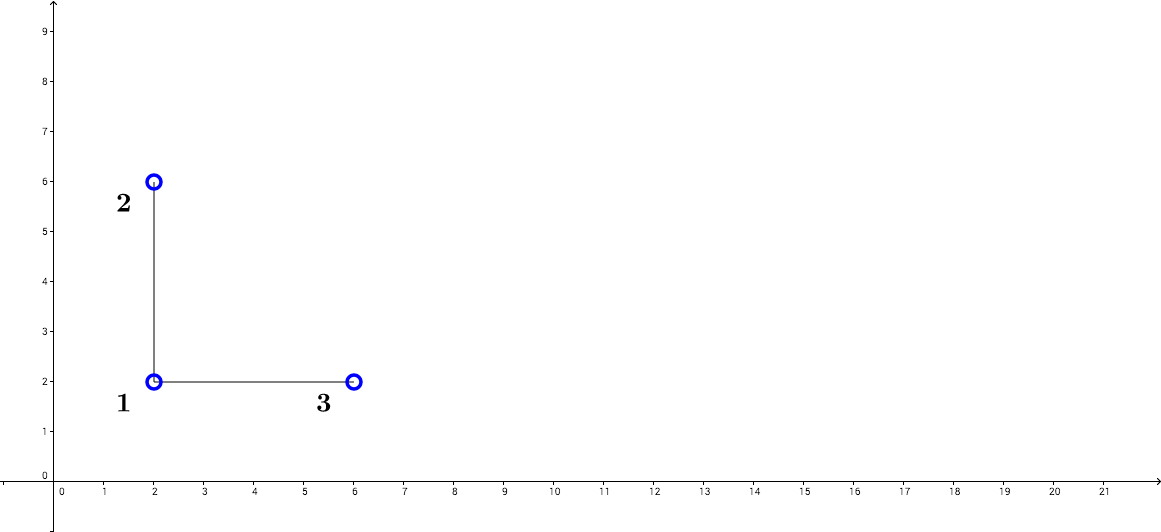
\includegraphics[scale=0.5]{grafEX.png}
	\end{center}
	\begin{align*}
		&\mathbf{E} = \{ \{1,2\}, \{1,3\}\}
		&& \mathbf{V} = \{1,2,3\}\\
		&\mathbf{A}_G = 
		\begin{bmatrix}
			0 & 1 & 1\\
			1 & 0 & 0\\
			1 & 0 & 0
		\end{bmatrix}
	\end{align*}
\end{Ex}
\begin{Ex}
	Riktad grad:
	\begin{center}
		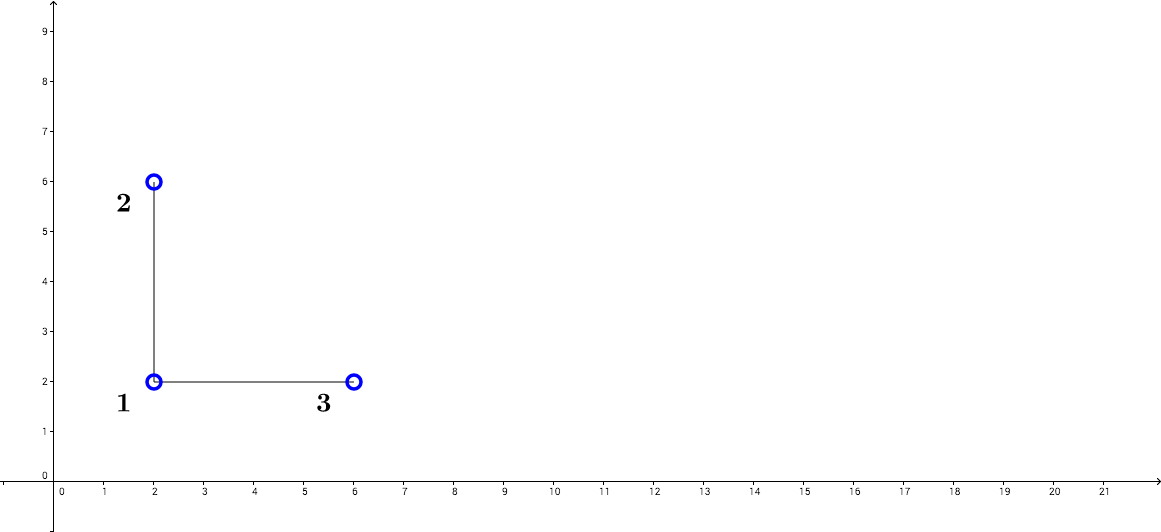
\includegraphics[scale=0.5]{grafEX.png}
	\end{center}
	\begin{align*}
		&\mathbf{E} = \{(1,2), (1,3)\}
		&&\mathbf{V} = \{1,2,3\}\\
		&\mathbf{A}_G = 
		\begin{bmatrix}
			0 & 1 & 1\\
			0 & 0 & 0\\
			0 & 0 & 0
		\end{bmatrix}
	\end{align*}
\end{Ex}
\begin{sats}
	Element (i,j) i grannmatris $\mathbf{A}_G^K$ ger antal vägar av längd \textit{k} från $v_i$ till $v_j$
\end{sats}
\begin{Ex}
	\[
	\mathbf{A}_G = 
	\begin{bmatrix}
		0 & 1 & 1\\
		1 & 0 & 0\\
		1 & 0 & 0
	\end{bmatrix}
	\]
	Beräkna antal vägar av längd 3.\\
	\textbf{Lösning:}
	\[
	\mathbf{A}_G \cdot \mathbf{A}_G \cdot \mathbf{A}_G = 
	\begin{bmatrix}
		0 & 2 & 2\\
		2 & 0 & 0\\
		2 & 0 & 0
	\end{bmatrix}
	\]
\end{Ex}
% section grafer (end)
\subsection{Övergångsmatris} % (fold)
\label{sec:section_name}
Om $\mathbf{A}_G$ är grannmatris till graf \textbf{G} med \textit{n} noder, så $\mathbf{M}_G$ övergångsmatris till \textbf{G} om:
\begin{align*}
&m_{ij} = a_{ij} / \sum\limits_{k = 1}^{n}a_{ik} 
&&\mbox{ $\mathbf{A}_G$ fast alla radsummor är 1}
\end{align*}

\begin{Ex}
	\begin{align*}
	& \mathbf{A}_G = 
	\begin{bmatrix}
		1 & 1 & 1\\
		1 & 0 & 0\\
		1 & 0 & 0
	\end{bmatrix}
	&& \mathbf{M}_G = 
	\begin{bmatrix}
		0 & 1/2 & 1/2\\
		1 & 0 & 0\\
		1 & 0 & 0
	\end{bmatrix}
	\end{align*}
\end{Ex}
Element på plats (i,j) i $\mathbf{M}_G^k$ är sannolikheten för att man befinner sig i nod $v_j$ efter \textit{k} steg om man startat i nod $v_i$
% section section_name (end)
\section{Slumpvandring} % (fold)
\label{sec:slumpvandring}
\begin{Def}
	Om vi befinner oss i en nod $v_i$ så beger vi oss till någon av dess grannar med sannolikheten $1/d(v_i)$, ($1/\mbox{antal grannar}$). Vi vill veta "vilken är sannolikheten att vara i en given nod vid en viss tidpunkt."
\end{Def}
Man studerar oftast slumpvandring med markovkedjor. 
\begin{Def}
	Låt $\vec{x}_o$ vara en startfördelning och låt en matris \textbf{P} vara en stokastisk matris (övergångsmatris). En markovkedja är en sekvens av fördelningsvektorer:
	\[
	\vec{x}_o, \vec{x}_1, \vec{x}_2, \vec{x}_3, ...
	\]
	Sådana att:
	\begin{align*}
	&\vec{x}_1 = \mathbf{P} \cdot \vec{x}_0
	&& \vec{x}_2 = \mathbf{P} \cdot \vec{x}_1
	&& \vec{x}_3 = \mathbf{P} \cdot \vec{x}_2
	&&.........
	\end{align*}
\end{Def}
\noindent
Övergångsmatrisen:
\begin{itemize}
	\item $\mathbf{P} = \mathbf{M}_G^T$ (alla kolumnsummor i \textbf{P} är 1). 
	\item I \textbf{P} kan förekomma andra element än $1/d(v_i)$.
	\item \textbf{P} har ofta element på diagonalen.
	\item \textbf{P} mpste vara en stokastisk matris. (Kolumnsummorna måste vara 1, och alla element $\ge 0$)
\end{itemize}
\begin{Ex}
	Utför slumpvandring på två websidor.
	\begin{center}
		Infoga exempelbild
	\end{center}
	\begin{itemize}
		\item Antag att $95\%$ att jag forsätter läsa \textcircled{1}, i nästa tidsteg, $5\%$ att jag byter till sida \textcircled{2}
		\item Antag att $97\%$ att jag forsätter läsa \textcircled{2}, i nästa tidsteg, $3\%$ att jag byter till sida \textcircled{1}
	\end{itemize}
	\begin{align*}
	&\mathbf{P} = 
	\begin{bmatrix}
		0.95 & 0.03\\
		0.05 & 0.97
	\end{bmatrix}
	\end{align*}
	Låt $\vec{x}_0 = \begin{bmatrix} 0.6\\0.4 \end{bmatrix}$ vara andel som läser sida \textcircled{1}, \textcircled{2} när vi börjar.
	\begin{gather*}
		\vec{x}_1 = \mathbf{P} = \vec{x}_0 = 
		\begin{bmatrix}
			0.95 & 0.03\\
			0.05 & 0.97
		\end{bmatrix} \cdot
		\begin{bmatrix} 0.6\\0.4 \end{bmatrix} = 
		\begin{bmatrix} 0.582\\0.418 \end{bmatrix} \\
		\vec{x}_2 = \mathbf{P} \cdot \vec{x}_1 = 
		\begin{bmatrix}
			0.95 & 0.03\\
			0.05 & 0.97
		\end{bmatrix} \cdot 
		\begin{bmatrix} 0.582\\0.418 \end{bmatrix} = 
		\begin{bmatrix} 0.565\\0.435 \end{bmatrix}\\
		\vdots \\
		\vec{x}_n = \mathbf{P} \cdot
		\begin{bmatrix}
			0.375\\
			0.625
		\end{bmatrix} = 
		\begin{bmatrix}
			0.375\\
			0.625
		\end{bmatrix}
	\end{gather*}
	Det kommer att kovergera. Stationär fördelning (steady state)\\
	Varje markovkedja med stokastisk matris har en stationär fördelning (steady state) $\vec{q}$ sådan att:
	\[
	\mathbf{P} \cdot \vec{q} = \vec{q}
	\]
	Dvs $\vec{q}$ är en egenvektor till \textbf{P} och $\lambda = 1$
\end{Ex}
\paragraph{Varför konvergerar markovkedjan?} % (fold)
\label{par:varf_r_konvergerar_markovkedjan_}
Vi beräknar egenvärden, egenvektorer till \textbf{P}
\begin{gather*}
	\lambda: \mathbf{det}(\mathbf{P} - \lambda \cdot \mathbf{I}) = 0
	\Leftrightarrow \mathbf{det}
	\begin{pmatrix}
		0.95 - \lambda & 0.03\\
		0.05 & 0.97 - \lambda
	\end{pmatrix} = ... = \lambda^2 -1.92 \lambda + 0.92 \Rightarrow
	\begin{cases}
		\lambda_1 = 1\\
		\lambda_2 = 0.92
	\end{cases}
\end{gather*}
Egenvektor:
\begin{gather*}
	(\mathbf{P} - 1 \cdot \mathbf{I}) = \emptyset \Rightarrow \vec{v}_1	=
	\begin{bmatrix}
		3\\5
	\end{bmatrix}\\
	(\mathbf{P} - 0.92 \cdot \mathbf{I}) = \emptyset \Rightarrow \vec{v}_2 = \begin{bmatrix} 1\\-1 \end{bmatrix}
\end{gather*}
\begin{gather*}
	\vec{x}_0 = c_1 \cdot \vec{v}_1 + c_2 \cdot \vec{v}_2\\
	\vec{x}_1 = \mathbf{P} \cdot \vec{x}_0 = \mathbf{P}(c1 \cdot \vec{v}_1 + c_2 \cdot \vec{v}_2) = c_1 \cdot \mathbf{P} \cdot \vec{v}_1 + c_2 \cdot \mathbf{P} \cdot \vec{v}_2 = c_1 \cdot \vec{v}_1 + c_2 \cdot 0.92 \cdot \vec{v}_2\\
	\vec{x}_2 = \mathbf{P} \cdot \vec{x}_1 = c_1 \cdot \mathbf{P} \cdot \vec{v}_1 + c_2 \cdot (0.92) \cdot \mathbf{P} \cdot \vec{v}_2 = c_1 \cdot \vec{v}_1 + c_2(0.92)^2 \cdot \vec{v}_\\
	\vdots\\
	\vec{x}_k = c_1 \cdot \vec{v}_1 + c_2 \cdot \overbrace{(0.92)^k}^\text{0 då $k \rightarrow \infty$} \cdot \vec{v}_2
\end{gather*}
% paragraph varf_r_konvergerar_markovkedjan_ (end)
% section slumpvandring (end)
\end{document}